\documentclass{article}

\usepackage{rotating}
\usepackage{graphicx}
\usepackage[utf]{inputenc}
\usepackage{url}
\title{Industrial Best Practice}


\begin{document}


\author{John Burchell \qquad William Granli \\
		john.a.burchell@gmail.com \qquad william.granli@gmail.com \\
		Computer Science and Engineering  \\
		University of Gothenburg }



\maketitle
\section{Executive Summary, 1p}
Do this last! 

\section{Problem Formulation, 3p}

\begin{itemize}
	\item Description of what problem you are trying to solve
	\item The description should highlight why the problem is important, for whom it is important and how it advances the state of the art/company business
	\item Description of similar solutions available for the market
\end{itemize}

\section{Roadmap and Plan, 5p}
\subsection{Designing the Roadmap}
Workshop 1 - Market
*Performance dimensions
*Market/business drivers
*Prioritisation
*Gaps

Workshop 2 - Product
*Product feature concepts
*Grouping
*Impact ranking
*Product strategy
*Gaps

Workshop 3 - Technology
*Technology solutions
*Grouping
*Impact ranking

Workshop 4 - Roadmapping
*Linking technology resources to future market opportunities
*Gaps


\begin{sidewaysfigure}[ht]
\centering
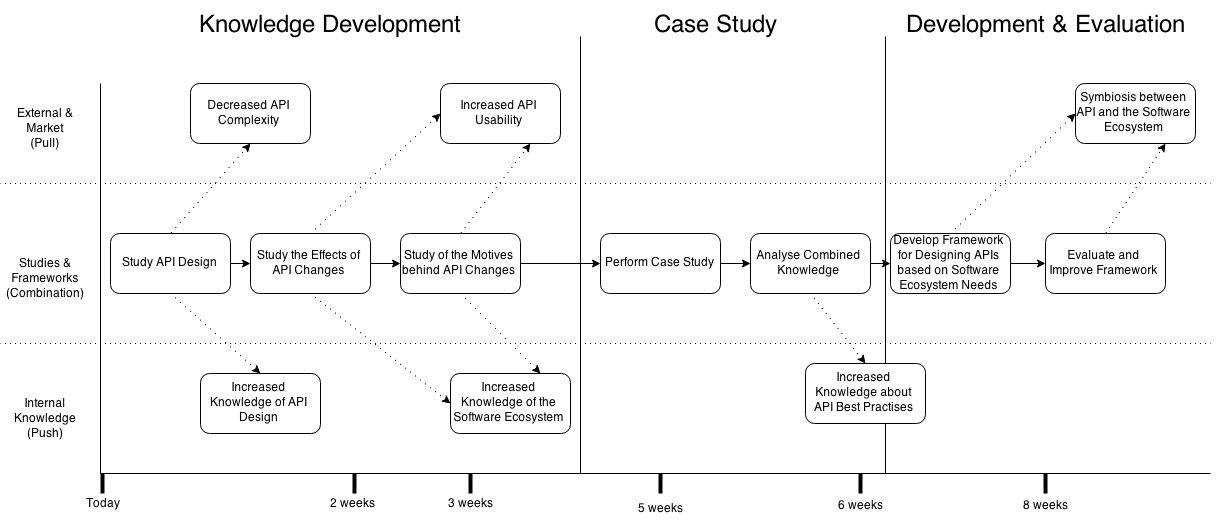
\includegraphics[width=220mm]{RoadMap.png}
\caption{The full lines denote in which way the organisation should ``logically'' view the roadmap. The dotted lines denote that one activity will lead to another. }
\end{sidewaysfigure}
%TODO: Add colours+graphix, extend dotted borders to left side as well, add x+y axes.

\begin{itemize}
	\item Description on how to solve the problem using a roadmap
	\item If the solution is a model – how to develop, implement, adopt, evaluate, etc.
	\item Project plan for the solution – the time scale can be thesis work or another project
\end{itemize}

\url{http://en.wikipedia.org/wiki/Technology_roadmap}

\section{Dissemination plan, 2p}

\begin{itemize}
	\item Description on how to present/sell the solution to the company
	\item Description on how to communicate the solution
\end{itemize}

\url{http://www.webarchive.org.uk/wayback/archive/20140614222502/http://www.jisc.ac.uk/fundingopportunities/projectmanagement/planning/dissemination.aspx}

\section{Impact assessment, 2p}


\begin{itemize}
	\item Description of how the solution advances the state of the art
	\item Description of how the solution advances the society in general (e.g. better cars, faster mobiles)
\end{itemize}

\url{http://en.wikipedia.org/wiki/Impact_assessment}


\section{Summary, 1p}

\begin{itemize}
	\item Account of how you can use the knowledge from the course in your further work
\end{itemize}




\end{document}